\chapter{Preliminaries}
In this section we will first present an example application that will be used throughout the report. Then, the paper about the original implementation of selective capture and replay by Joshi and Orso \cite{orso05may} will be summarized.


\section{Example Application}
In the following we will present our example application. It will be explained in detail here and then be used throughout this report.

Consider a customer that wants to withdraw money from his account. He interacts with the user interface at an ATM (\figref{fig:example_class_diagram}). This user interface could be implemented in different ways (textual or graphical). The transactions that the customer executes at the user interface are first written to the ATM's journal and then dispatched to the bank. When the customer wants to withdraw money, the bank withdraws money from the customers bank account and the ATM then hands the money to the customer.
 \begin{figure}[ht]
   \centering
   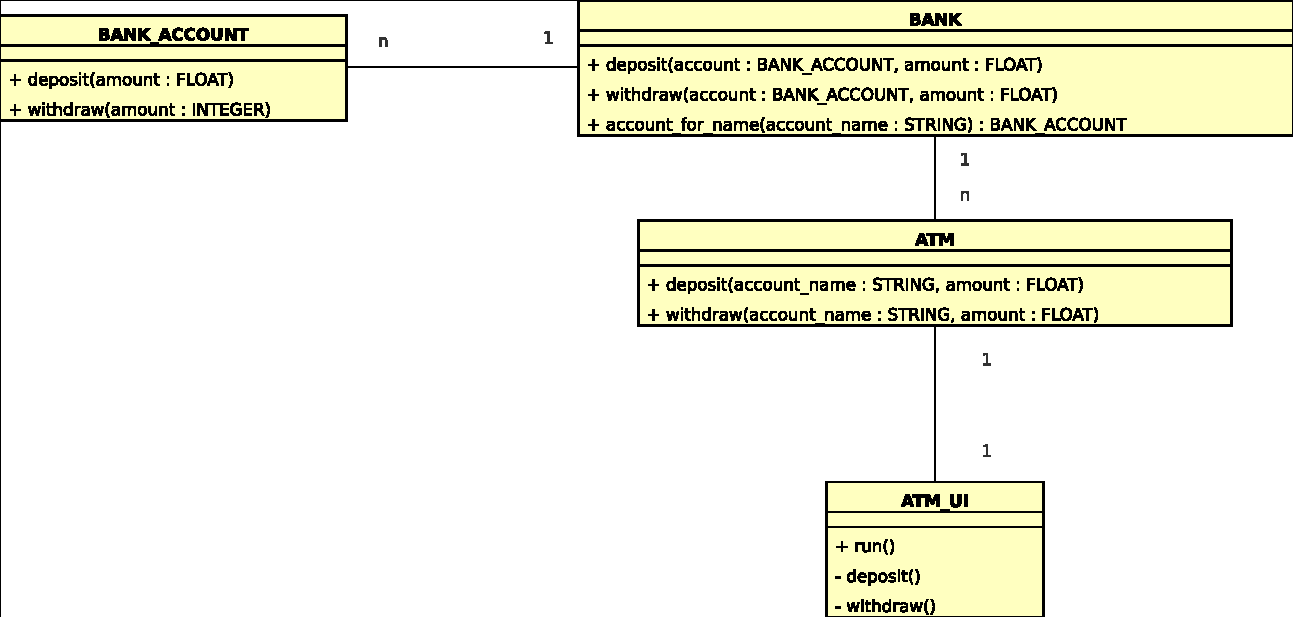
\includegraphics[width=1\textwidth]{illustrations/example_class_diagram}
   \caption{Class Diagram showing the example of a Bank and ATMs}
   \label{fig:example_class_diagram}
\end{figure}

Note that the names of classes and methods were apply to the style presented in Object Oriented Software Construction, second edition \cite{oosc2}. Even Java examples that refer to this application will use that style to keep the same class and method names.

\begin{figure}[ht]
   \centering
   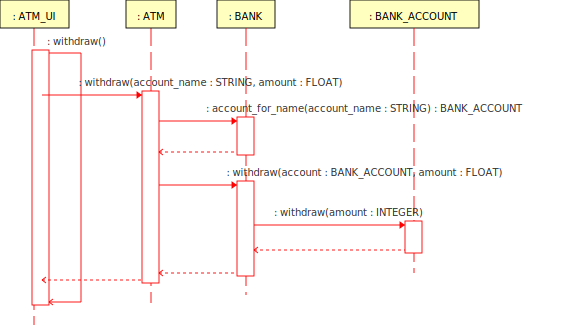
\includegraphics[width=1\textwidth]{illustrations/example_withdrawal}
   \caption{Sequence Diagram of a Withdrawal Operation Invoked by the Customer}
   \label{fig:example_withdraw_sequence}
\end{figure}

One use case is money withdrawal by a customer via an ATM. The customer launches the withdrawal operation on the \class{ATM\_UI}. The request is passed through the \class{ATM} to the \class{BANK} which then withdraws the money from the Account. The sequence diagram (\figref{fig:example_withdraw_sequence}) should clarify how the classes interact with each other.



\section{Selective Capture and Replay}
After giving the overview about the different capture and replay techniques in the related work chapter	, our choice will be described here in detail. Currently there exist two implementations of selective capture and replay, both for Java: SCARPE \cite{orso05may, orso06}, the original implementation, and JINSI \cite{JINSI}, which minimizes failure inducing component interactions that were captured using selective capture and replay.

This chapter summarizes papers from Joshi and Orso about original implementation of selective capture and replay (SCARPE) \cite{orso05may, orso06}. Where appropriate, some examples using the application described before are introduced.

\subsection{Technique and Terminology}

\begin{figure}[ht]
  \centering
  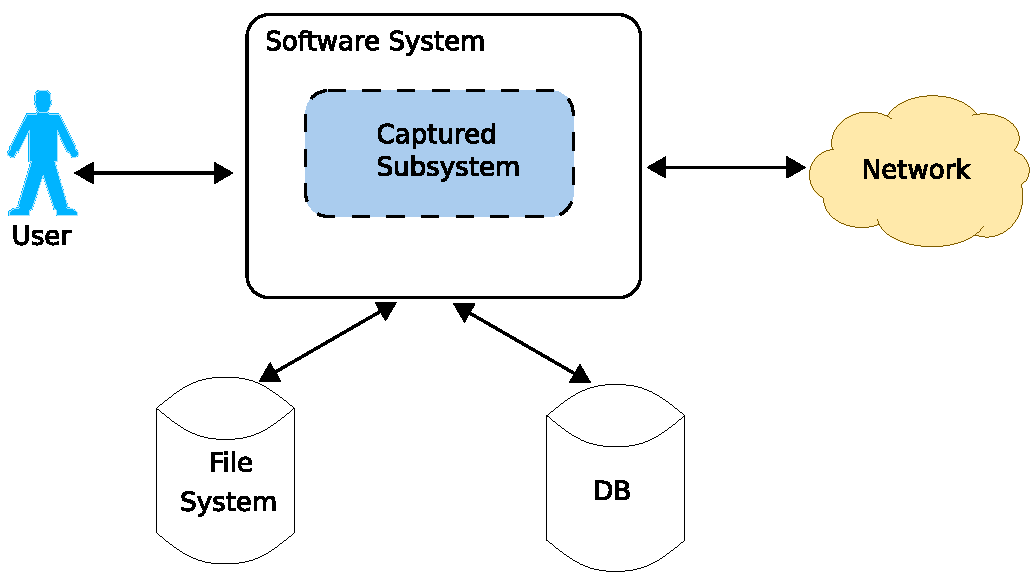
\includegraphics[width=1\textwidth]{illustrations/scr_overall_schema}
  \caption{System Layout of the Example Application Showing the Captured Subsystem (derived from Joshi and Orso \cite{orso05may})}
  \label{fig:scr_overall_schema}
\end{figure}

This technique lets the user choose the subset of the program that should be captured and replayed (\emph{captured subsystem}, \figref{fig:scr_overall_schema}). It then only captures the execution data of that subsystem, ignoring the other parts of the system. The relevant interactions between the captured subsystem and the outside world is captured in terms of events; those events are read during the replay phase in order to replay the corresponding interactions. Only the essential part of the information that traverses the border between the captured subsystem and the rest of the system is captured. This is a significant improvement over other existing techniques that capture all the data, especially when big datastructures are passed over the border and only a part of those datastructures is actually accessed.

Here are some terms that are used to describe selective capture and replay:
\begin{description}
	\item [The observed set] is the subsystem that was selected for capture and replay.
	\item [The observed classes] are the classes in the observed set. Observed code is defined analogously.
	\item [Observed methods and fields] are the fields and methods of the observed classes.
\end{description}
\emph{Unobserved set},  \emph{unobserved classes}, \emph{unobserved code}, \emph{unobserved methods} and \emph{unobserved fields} are the corresponding terms for the part of the system that was not selected for capture and replay.
\begin{description}
	\item [External code] denotes either unobserved or library code.
	\item [Unmodifiable classes] are the classes whose code can not be modified (e.g. some system classes such as \identifier{java.lang.Class}) due to constraints from the Java Virtual Machines
	\item [Modifiable classes] are all classes except the \emph{unmodifiable classes}
\end{description}

The technique is divided in two main phases: capture and replay. \figref{fig:scr_capture_replay_phase} illustrates the setup of of these two phases in selective capture and replay.
\begin{figure}[ht]
  \centering
  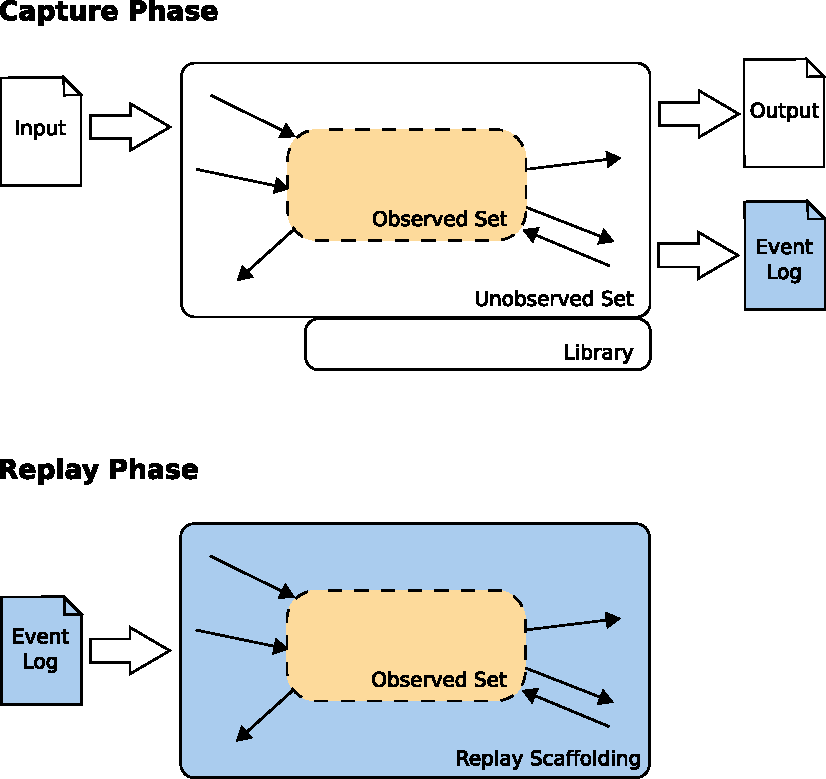
\includegraphics[width=0.8\textwidth]{illustrations/scr_capture_replay_phase}
  \caption{Capture and Replay Phase in Selective Capture and Replay (derived from Joshi and Orso \cite{orso05may})}
  \label{fig:scr_capture_replay_phase}
%\includegraphics{illustrations/capture_and_replay_generic_structure}
\end{figure}
The \emph {capture phase} takes place when the application is run for recording. Before the application starts, the boundaries of the observed set are identified and the application is instrumented in order to be able to capture interactions between the observed set and the rest of the system. While the application runs, the instrumentation generates the events for these interactions and writes them to the \emph{event log}.

In the \emph{replay phase}, the technique generates the \emph{replay scaffolding}. The replay scaffolding uses the event log to replay the events on the observed set. Replaying consists both of performing actions on the observed set (e.g. invocation of a method of the observed set) and consuming actions of the observed set (e.g. receiving a method invocation originally targeted to the unobserved set), thus the replay scaffolding acts both as a driver and stub.

\subsection{Capture Phase}
The capture phase is used to gather the necessary information to replay the application afterwards. In the following we will show how SCARPE \cite{orso05may} gathers that information.

\subsubsection{Capturing Partial Information}
To see the need for a solution of not capturing the whole data that flows over the border clearer, consider the case when a bank tries to find out the time of the last journal entry of an ATM. Assume that the classes \class{BANK} and \class{BANK\_ACCOUNT} belong to the observed set and the rest of the application belongs to the unobserved set. The following instructions access the atm's journal and print the time of the last journal entry:

\javalisting
\begin{lstlisting}
 ATM_JOURNAL journal = atm.journal
 print (journal.time_of_last_entry)
\end{lstlisting}

\class{ATM\_JOURNAL} can contain a thousand of journal entries. In a traditional approach, due to the access to the journal, the whole data structure including all journal entries would be serialized each time the journal is accessed. The idea of selective capture and replay is to only write the referenced object that was passed (the journal) to the event log. When later \class{BANK} accesses the method \feature{time\_of\_last\_entry}, the result is again written to the event log, because the access crosses the border: from \class{BANK} (observed) to \class{ATM\_JOURNAL} (unobserved). This reduces the size of the event log significantly, because only the the data that is used needs to be written down.

The technique for capturing only partial information instead of the whole data that flows into unobserved set relies on \emph{object IDs}. An object ID uniquely identifies a class instance. SCARPE introduces the object ID into the program by adding an additional field to all modifiable classes. It further instruments the creation constructors of these classes so that the unique object ID is acquired from a global counter. For unmodifiable classes however, a reference map is needed to store the object ID of its instances. The object ID for instances of unmodifiable classes is acquired when it is looked up the first time. The reference map uses weak references so that the referenced objects can be collected by the garbage collector to avoid memory leaks.

Instead of recursively serializing the data that crosses the boundaries of the observed set, selective capture and replay only records a small part:
\begin{itemize}
 \item Scalar values (values of a basic type) are fully captured.
 \item For objects, the technique only captures the object ID and the type. The type is used to restore the object again during replay phase.
\end{itemize}

Although the rules for this approach are simple, it is not obvious that they suffice to replay an application. Therefore we provide a short reasoning of why this works:

%TODO: bei jedem Punkt 1 Szenario.
\begin{enumerate}
  \item [1)] Instances of observed classes are fully populated during replay, because all actions from the unobserved set are replayed on them and the actions from the observed set are executed on them as in the original run.
  \item [2)] During replay, observed code accesses to methods or fields can either return instances of observed classes or instances of unobserved classes.
  \item [3)] When an object of an observed class is returned, it is fully populated due to 1) and therefore its fields and methods can safely be accessed.
  \item [4)] When an object of an unobserved class is returned, each further access to a field or method from observed code to that object would result in the capturing of another boundary crossing event. Therefore the results of these accesses can be reconstructed during replay.
  \item [5)] Therefore, it is assured that during replay, it is possible for the observed code to access the fields and methods like it did in the original run.
\end{enumerate}



\subsubsection {Interactions between Observed and External Code}
Method calls are an elementary way to communicate between observed and external part of the application. The technique captures calls in both directions: from observed to unobserved code and vice versa. The following events are related to method calls:

%TODO: Beispiel zu jedem event einführen!

\begin{description}
 \item  [OUTCALL] events that represent calls from observed code to unobserved methods.
 \item [INCALL] events that represent calls from unobserved code to observed methods.
 \item [OUTCALLRET] events for the return from outcalls
 \item [INCALLRET] events for the return from incalls
\end{description}

OUTCALL and INCALL events (\emph {call events})  have the same attributes:

\begin{description}
 \item [Receiver] The receiver object
 \item [Method called] Signature of the called method.
 \item [Parameters] The list of scalar values and objects passed to the method.
\end{description}

Capturing of call events involves capturing of scalar values and objects. They are written to the log as follows:

%TODO: log example zeigen:
\begin{description}
 \item [Scalar values] are written verbatim to the log.
 \item [Objects] are written by storing their type and object ID. For null values, the object ID is set to zero. 
\end{description}

OUTCALLRET and INCALLRET events (\emph{callret events}) have only one attribute: the returned value.

OUTCALL and OUTCALLRET events are captured by instrumenting the observed code. A probe is added to all calls to external methods. It is not always possible to distinguish calls to observed code from calls to unobserved code, as we will discuss later.

To capture INCALL and INCALLRET events, proxy methods are introduced in a way that makes it unnecessary to instrument external code. It is ensured that calls inside the observed code don't call these proxy methods but the actual methods. Thus calls from observed code to observed methods can be executed without overhead.

Field Accesses are another source of interaction between observed and external classes. Read accesses from unobserved to observed code don't influence the execution behaviour of the observed code therefore they are not captured. Thus three kinds of events are recorded:

\begin{description}
 \item [OUTREAD] events are generated when observed code reads the content of an unobserved field.
 \item [OUTWRITE] events denote write accesses from observed code to unobserved code.
 \item [INWRITE] events are write accesses from unobserved code to observed code.
\end{description}

OUTREAD, OUTWRITE and INWRITE have the same attributes:

\begin{description}
 \item [Receiver:] The object whose field is accessed.
 \item [Field Name:] The name of the field that is accessed.
 \item [Value:] The read or written value.
\end{description}

OUTREAD and OUTWRITE events are captured by adding probes in the observed code where fields of external classes are accessed. INWRITE events are captured in the same way, but here the unobserved code is instrumented whenever an observed field is written. 

Exceptions are another interaction mechanism that needs to be considered for capture and replay. Because exceptions were not implemented in our Eiffel implementation of selective capture and replay, they will be treated only briefly. For exceptions two more types of events were introduced:
\begin{description}
 \item [EXCIN] events are for exceptions that propagate from the external to the observed code.
 \item [EXCOUT] events are for exceptions that propagate from the internal to the external code.
\end{description}
EXCOUT events are captured by wrapping all observed methods with a \identifier{try\--catch} block. By wrapping instructions that call an observed method with an exception handler,  EXCIN events are captured.

\subsection{Replay Phase}
During the replay phase, the observed code is re-executed based on the event log that was gathered during the capture phase. Before replaying the observed code, selective capture and replay instruments the code based on the interactions between observed and external code. 

\subsubsection{Object Creation}
In the replay phase, object IDs are treated in a different way. Now it is necessary to find the object that matches a given object ID, not reverse. In order to allow this resolving, the technique uses a reference map that maps the object ID to all available  objects. The technique extracts the object IDs from the event's attributes and then retrieves the associated object or creates it. How these objects are created depends on whether they are instances of observed or external classes.
\begin{description}
 \item [Instances of External Classes:] For external classes, \emph{placeholder objects} are created. These objects have the correct type in order to support reflection in the observed code (e.g. \identifier{instanceof}), but their state is irrelevant. After creation, the objects are registered in the reference map.
 \item [Instances of Observed Classes:] Instances of observed objects are either created automatically by the observed code or there must be an INCALL event to the constructor in the event log. When replaying an INCALL to a constructor, an entry for the object is added to the reference map.
 \item [Null Values] If the object ID is zero, \identifier{null} is returned.
\end{description}

\subsubsection{Event Replaying}
For the replay phase, a scaffolding is generated that imitates the behaviour of the external code, thus behaves both as a driver and stub. Whenever control returns to the scaffolding, it checks whether the received event matches the next event in the log. If the events don't match (\emph{out-of-sync events}), a message is displayed to the user, who can chose whether to ignore the discrepancy and continue, or stop the replay.  Out-of-sync events can only occur, if the code was changed between capture and replay phase, for example because the technique is used for regression testing. If the events from log and replay match, the event in the log is  consumed and replay continues. Otherwise the technique asks the user whether he wants to abort or skip the unmatched event and continue.

In contrast to INCALL, INWRITE, OUTREAD, OUTCALLRET and EXCIN, which are necessary to replay the observed code correctly, OUTCALL, INCALLRET, OUTWRITE, EXCOUT are not necessary to replay the observed code, but they can be used as oracles for regression testing. The observed set is considered to be the system under test, which generates OUTCALL, INCALLRET, OUTWRITE and EXCOUT events as output, these events can then be compared to the recorded events of the capture phase - the recorded events are used as oracle.

\begin{description}
%TODO: example einweben!
 \item [INCALL Events] To replay INCALL events, the method first retrieves the target object from the reference map. If the target object is not in the reference map, it must be either a call to a constructor or a static call. Then, it retrieves the parameters from the reference map, or creates the scalar values corresponding to the parameters. If the object can't be retrieved from the reference map, a placeholder object is created. Then, the technique can call the specified method with all arguments; the control flows to the observed code. 
 \item [INCALLRET Events] INCALLRET events are not essential for replaying the observed code. They occur as a result of INCALL events and are consumed by the replay scaffolding. To ensure a correct replay, the scaffolding checks if returned value conforms to the one of the next event in the event log.
 \item [OUTCALL Events] All invocations to unobserved methods from the observed code are replaced by two instructions: (1) The call to a special feature in the scaffolding (\identifier{consumeCall}) and (2) The assignment of the result of the invocation. For example \inlinejava{TIME t = atm_journal.time_of_last_entry()}, with TIME and ATM\_JOURNAL both being in the package \identifier{foo}, would be replaced by the following instructions:
\begin{lstlisting}
 Object tmp = scaffolding.consumeCall("foo/ATM_JOURNAL",
                24,/*object ID for atm_journal*/
                "time:()Lfoo/TIME",
                {} /*empty array of parameters*/
		);
 TIME t = (TIME) tmp;
\end{lstlisting}
The scaffolding checks whether type, parameters, target and methodname of the next event from the log matches to the reported call. If the events match, then replay continues with the next event, otherwise an error is reported to the user.
 \item [OUTCALLRET Events]As these events occur as a result of OUTCALL events, they are treated within \feature{consumeCall}. The method looks up the return value in the event log and retrieves it using the reference map. 
 \item [OUTREAD and OUTWRITE Events] To replay these events, accesses to unobserved fields are instrumented in the observed code, by calling associated methods from the scaffolding, \feature{consumeRead} for OUTREAD events and \feature{consumeWrite} for OUTWRITE events. For example the instruction \class{ATM\_JOURNAL journal = atm.journal}, with \class{ATM\_JOURNAL} and \class{ATM} both belonging to package \identifier{foo}, would be replaced by the following instruction:
\begin{lstlisting}
 ATM_JOURNAL journal = scaffolding.consumeRead ("foo/ATM",
                24,/*Object ID for atm*/
                "val")
\end{lstlisting}
The methods \feature{consumeRead} and \feature{consumeWrite} check if the event from the log matches the detected one. The method \feature{outRead} furthermore returns value associated with the event.
 \item [INWRITE Events] In order to replay an INWRITE event, the scaffolding retrieves the target, the name of the field that should be modified and the value to be assigned. It resolves the target, which must exist unless it is a static field access. The value to be assigned is resolved as well or created if it does not exist yet. Finally the scaffolding sets the field of the target to the specified value.
 \item [EXCIN and EXCOUT Events]  To replay EXCIN events, the method \feature{consumeCall} creates and throws a corresponding exception. This is possible, because EXCIN events can only occur during an outcall. EXCOUT events, which are generated by the observed code, are caught by the replay scaffolding and compared to the next event in the event log. If the exception matches the event from the event log, replay continues.
\end{description}

\subsubsection{Assumptions}
The following list of assumption are required for selective capture and replay:
\begin{itemize}
 \item It is assumed that there is no direct access from unmodifiable classes to fields of observed classes.
 \item Because native code is not instrumented, Joshi and Orso also assume that there is no direct access from native code to observed fields.
 \item The technique can not guarantee the same thread schedule during capture and replay phase. Therefore it is assumed that the interleaving due to multi-threading does not change the behaviour of the observed code.
 \item The technique assumes that runtime exceptions occur deterministically. This is necessary, because exceptions generated in the observed code are consumed, but not replayed.
\end{itemize}

\subsubsection{Special Cases}
There are some special cases that need to be considered when implementing selective capture and replay:

%TODO: Beispiele einfüge!
\begin{description}
 \item [Polymorphism and Dynamic Binding] It is not always possible to determine whether an event is internal or external, when it depends on the dynamic type of the receiver. In these cases, it is necessary to add a runtime check to determine whether the receiver is an internal or external class, which is done using the \identifier{instanceof} operator. We assume that this case occurs at least in examples that use multiple interface inheritance, where it can not be assumed that the implementers of an interface are either all in the observed set or all in the unobserved set.
 \item [Inheritance] If a class \identifier{c} is in the observed set, but not all of \identifier{c}'s subclasses, creating an instance of any of \identifier{c}'s subclasses would result in the creation of an instance of \identifier{c}. To avoid this issue, it is required that if a class \identifier{c} is added to the observed set, all subclasses of \identifier{c} are also in the observed set. We assume that problem described here is implementation specific, and could be avoided.
 \item [Reflection] The technique handles most cases of reflection, however in some cases, additional instrumentation is required (e.g. if reflection is used in external code to modify fields of observed classes). 
 \item [Access Modifiers] In order to replay recorded executions, in some cases it is necessary to change access modifiers. We assume that this applies primarily to the \identifier{protected} modifier, which may prohibit access to observed classes from within the replay scaffolding.
 \item [Garbage Collection] To allow the collection of unused objects, the technique must make sure that it does not keep references to unused objects. For example the reference map must use weak references to avoid memory leaks.
 \item [Finalize] Calls to \identifier{finalize} are non-deterministic in Java, thus they can generate out-of-sync events during the replay phase. Therefore calls to \identifier{finalize} are treated in a special way: when receiving a call to \identifier{finalize}, the technique consumes the next matching entry in the event log, that is a call to \identifier{finalize}.
\end{description}
